\section{Norm penalities}
We denote the regularized objective function by:
\begin{center}
    $\tilde{J}(\bm{\theta}, \bm{X}, \bm{y}) = J(\bm{\theta}, \bm{X}, \bm{y}) =
    \alpha\Omega(\bm{\theta})$ with 
    $\begin{cases}
        \alpha\in[0,\infty[\text{ hyper-parameters weighting the impact of norm 
        penalty}\\
        \Omega\text{ relative to standard objective function }J
    \end{cases}$
\end{center}

% \subsection{$L^{2}$ parameter regularization}
\paragraph{Purpose}: This penalty is as well knows as \tB{weight decay}, it allows
to drives the weight closer to the origin.

\paragraph{Theory}
$\Omega(\bm{\theta}) = \dfrac{1}{2}\norm{\bm{w}}^{2}_{2}$

\subsection{Data Augmentation}

\subsection{Drop out}
\paragraph{Purpose}
It provides an inexpensive approximation to \tB{training and evaluating a \emph{bagged
ensemble} of exponentially many neural networks}.

\paragraph{Theory}
It \uB{trains the ensemble consisting of \textbf{all sub-networks that can be formed by
removing non-output units}} from an underlying base network.
\begin{figure}[H]
    \begin{center}
        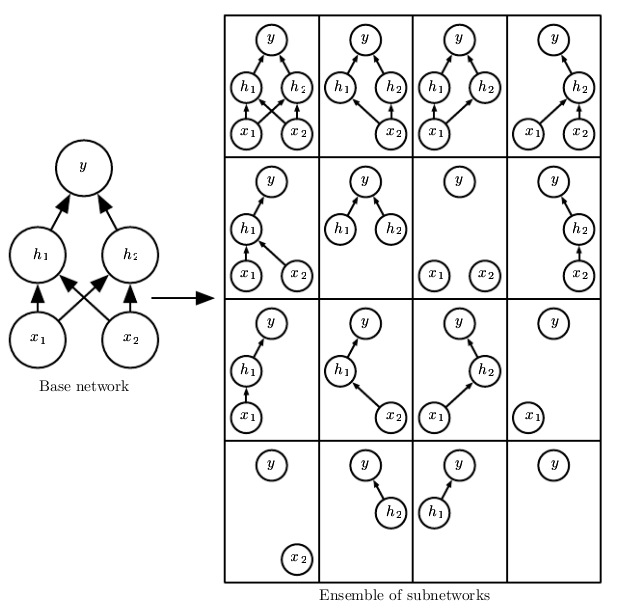
\includegraphics[width=.5\textwidth]{chapters/4_deep_learning/2_regularization/images/01_droupout.png}
    \end{center}
    \caption{Drop out illustration}
    \label{fig:01_droupout.png}
\end{figure}



